\documentclass[11pt]{article}
\usepackage[T1]{fontenc}
\usepackage[left=12mm,
right=12mm,top=1.5in,
bottom=1.5in]{geometry}
\usepackage{mathtools}
\usepackage{cancel}
\usepackage{graphicx}
\usepackage{grffile}
\graphicspath{{/home/piotr/Documents/scientific-computing/list04/exercise5/plots/}{/home/piotr/Documents/scientific-computing/list04/exercise6/plots/}}
\DeclareUnicodeCharacter{2212}{-}
\begin{document}
\title{{Obliczenia Naukowe}}
\author{Laboratorium Lista Nr 5\\Piotr Popis\\ 245162}
\date{6 grudzień 2019}
\maketitle
\centering

\begin{flushleft}
\section{Zadanie 1}
\bigskip
\subsection{Opis problemu}
\bigskip
Celem zadania jest implementacja funkcji obliczającej ilorazy różnicowe. Danymi wejściowymi są:
\begin{center}
x- wektor długości n+ 1 zawierający węzły $x_0, . . . , x_n$  $x[1]=x_0,...,x[n+1]=x_n$\\
f– wektor długości n+1 zawierający wartości interpolowanejfunkcji w węzłach $f(x_0), . . . , f(x_n)$\\
\begin{flushleft}
Wyniki:
\end{flushleft}
fx- wektor długości $n+1$ zawierający obliczone ilorazy różnicowe\\ $fx[1]=f[x_0]$,\\$fx[2]=f[x_0, x_1],...,fx[n]=f[x_0, . . . , x_{n−1}],fx[n+1]=f[x_0, . . . , x_n].$
\begin{flushleft}
Addytywnym utrudnieniem jest restrykcja użycia tablicy dwuwymiarowej, czyli macierzy.
\end{flushleft}
\end{center}
\subsection{Rozwiązanie}
Ilorazem różnicowym n- tego rzędu funkcji $f:X\longrightarrow Y$ w punktach $x_0, ..., x_n \epsilon X$ nazywamy funkcję:\\
\begin{center}
$$f(x_0,...,x_n) := \sum^n_i\dfrac{f(x_i)}{\prod_j^n (x_i-x_j)}$$
\end{center}
\newpage
\bigskip
W celu realizacji zadania, czyli uniknięcia wykorzystania macierzy skorzystamy z zależności rekurencyjnej:\\
\bigskip
1.$i=0$\\
\quad$f[x_0]=f(x_0)$\\
\bigskip
2.$i=1$\\
\quad$f[x_0,x_1]=\dfrac{f(x_1)-f(x_0)}{x_1-x_0}$\\
\bigskip
3.$i=n$\\
\quad$f[x_0,...,x_n]=
\dfrac{f(x_1,...,x_n)-f(x_0,...,x_{n-1})}{x_n-x_0}$\\
\bigskip
Znając węzły $x_n$ i wartości funkcji f($x_n$), można utworzyć dwuwymiarową tablicę ilorazów różnicowych. Jednak prowadzi to do źle uwarunkowanej macierzy Vanermode'a. Algorytm natomiast można zoopytmalizować, ponieważ wystarczy użyć tablicy jednowymiarowej $w$ do zapamiętywania dwóch poprzednich wartości(tablicę aktualizujemy od góry do dołu i od lewej do prawej). Pozostałe wartości są po prostu niepotrzebne. Początkowymi wartości $w_i$ są odpowiadające im f[$x_i$]. Ostatecznie ilorazem różnicowym opartym na węzłach $x_0,...,x_n$ będziemy nazywali wielkość $f[x_0,...,x_n]$.\\
\bigskip
Postać Newton'a wzoru interpolacyjnego\\
\bigskip
$$p(x)=\sum^n_{k=0}c_kq_k(x)=\sum^n_{k=0}f[x_0,...,x_k]\prod^{k-1}_{j=0}(x-x_j)$$\\
\bigskip
\quad gdzie $c_0$ zależy od f($x_0$), \\
\begin{center}
.\\.\\.\\
\end{center}
\quad $c_n$ zależy od f w punktach $x_0,...,x_n $\\
\bigskip
\newpage
\section{Zadanie 2}
\subsection{Opis problemu}
Napisać funkcję obliczającą wartość wielomianu interpolacyjnego stopnia n w postaci Newtona $N_n(x)$ w punkcie x=t za pomocą algorytmu Hornera w czasie $\theta(n)$. Dane wejściowe:\\
\begin{center}
x– wektor długości n+ 1 zawierający węzły $x_0, ...,x_n$\\$x[1]=x0,...,x[n+1]=x_n$\\
fx– wektor długości n+ 1 zawierający ilorazy  różnicowe \\$fx[1]=f[x_0]$,\\
$fx[2]=f[x_0, x_1],...,fx[n]=f[x_0, . . . , x_{n−1}],fx[n+1]=f[x_0, . . . , x_n]$
\end{center}
\begin{flushleft}
Wyniki:
\begin{center}
a – wektor długości n+ 1 zawierający obliczone współczynniki postaci naturalnej\\
$a[1]=a_0$,\\
$a[2]=a_1,...,a[n]
=a_{n−1},a[n+1]=a_n$.\\
\end{center}
\end{flushleft}
\subsection{Rozwiązanie}
W celu wyznaczenia wartości wielomianu interpolacyjnego stopnia n w postaci Newton'a $N_n(x)$ w punkcie $x=t$ zaimplementowano uogólniony schemat Hornera.\\
\begin{center}
$$N_n(x)=\sum^k_{i=0}c_i\prod^{i-1}_{j=0}(x-x_j)$$
\end{center}
Wartość wielomianu przyjmowana w danym punkcie t obliczamy, kosztystając z:\\
\begin{center}$w(x)=(x-t)\cdot q(z)\cdot w(t)$\end{center}
Można też śmiało stwierdzić, iż metoda Newton'a jest trudniejsza w impementacji niż np metoda Lagrange'a i wymaga większej ilości oddzielnych kroków. Jest jednak znacznie lepiej uwarunkowana nmerycznie.W metodzie najpierw wzynaczane są odpowiednie ilorazy różnicowe, a dopiero później z ich użyciem- interpolowa funkcja.\\
Algorytm zaczynamy od przypisania do zmiennej nt konkretnego wektora ilorazów różnicowych. W kolejnych krokach od n-1 zwiększamy wartość wektora pomnożoną przez różnicę wartości węzła i weilomianu t. Otrzymujemy:\\
\begin{center}
$nt=f_x(i)+nt\cdot (t-\omega[i])$, gdzie $f_x$ jest wektorem ilorazów różnicowych.\\
\end{center}
Algorytm działa w czasie liniowym.
\newpage
\section{Zadanie 3}
\subsection{Opis Problemu}
Celem zadania jest kreacja funkcji obliczającej współczynniki postaci naturalnej wielomianu interpolacyjnego znając współczynniki wielomianu interpolacyjnnego w postaci Newton'a $c_0$ = f[$x_0$], $c_1$ = $f[x_0,x_1]$, $c_2$= $f[x_0, x_1, x_2],. . .,cn=f[x_0, . . . , x_n]$ (ilorazy różnicowe) oraz węzły $ x_0, x_2, . . . , x_n $ działającą w czasie $\theta(n^2)$. Dane wejściowe:\\
\begin{center}
x– wektor długości $n+ 1 $ zawierający węzły $x_0, . . . , x_n x[1]=x_0,...,x[n+1]=x_n$ \\
fx– wektor długości n+ 1 zawierający ilorazy różnicowe $fx[1]=f[x_0],fx[2]=f[x_0, x_1],...,fx[n]=f[x0, . . . , x_{n−1}],fx[n+1]=f[x0, . . . , x_n]$\\
\begin{flushleft}
Wyniki:\\
\end{flushleft}
a– wektor długości $n+ 1 $ zawierający obliczone współczynniki postaci naturalnej\\
$a[1]=a_0$,\\
$a[2]=a_...,a[n]=a_{n−1},a[n+1]=a_n$
\end{center}
\bigskip
\subsection{Rozwiązanie}
\bigskip
Korzystając z faktu, iż współczynnik sąsiadujący z $x^k$ to f[$x_0,x_1,...,x_k$], czyli $c_n$ przy najwyżej potędze wielomianu w postaci Newton'a. Ponownie wykorzystujemy ugólnienie schematu Hornera, a następnie z wzoru na postać Newton'a podanego na  wykładzie: \\
\begin{center}
\bigskip
$$p(x) = \sum_{k=0}^n f[x_0,...,x_k] \prod^{k-1}_{j=0}(x-x_j)$$\\
\bigskip
\end{center}
Wielomian posiada współczynniki przy odpowiadających im potęgach $a_0,a_1,...,a_k$, gdzie współczynnik $a_k$ leży przy największej potędze. Dokonujemy mnożenia danego wielomianu począwszy od jego ostatnich potęg. W każdym kroku mnożemy nasz  wielomian przez dwumian $(x-x_{n-1})$. Ostateczny wielomian wynikowy będzie zaprezentwoany jako prosty wektor współczynników analagoiczny do wektora wejściowego. W wyniku wykonanych mnożeń otrzymujemy postać wynikową wielomianu, którego współczynniki wynoszą kolejno $a_k,a_{k-1},..,a_0$. Aby wynik był postaci $a_0+a_1x+a_x^2+...+a_nx^n$ musimy dokonać również przestawienia. Całkowita złożoność obliczeniowa wynosi $\theta(n^2)$, ponieważ złożoność obliczeniowa schmeatu Horner;a wynosi $\theta(n)$ oraz mnożenie wielomianów również $\theta(n)$
\newpage
\section{Zadanie 4}
\subsection{Opis Problemu}
Celem zadania jest utworzenie funkcji, która zinterpoluje zadaną funkcję f(x) w przedziale [a,b] za pomocą wielominau interpolacyjnego stopnia n w postaci Newton'a, a następnie narysuje wielomian interpolacyjny i funkcję interpolową. Wykorzystać Plots lub PyPlot lub Gadfly do narysowania grafów.\\
\quad W interpolacji użyć węzłów równoodległych, \\
\bigskip
\quad\quad$x_k=a+k\cdot h$,\\
\quad\quad $h =\dfrac{b-a}{n}, k = 0,1...,n$\\
W zadaniu należy nie wyznaczać jawnej postaci wielomianu interpolacyjnego. Należy skorzystać z funkcji zaimplementowanych w zadaniu 1 oraz zadaniu 2 odpowiednio iloryRzonicowe i warNewton. Dane wejściowe:\\
\begin{center}
f– funkcja f(x) zadana jako anonimowa funkcja,\\
a,b– przedział interpolacji, 
\\n– stopień wielomianu interpolacyjnego
\begin{flushleft}
Wyniki:
\end{flushleft}
-funkcja rysuje wielomian interpolacyjny i interpolowaną funkcję w przedziale[a, b]
\end{center}
\bigskip
\subsection{Rozwiązanie}
\bigskip
Pierwszym schodem jest wyznaczenie równoodległch węzłów i obliczenie odległosci h między nimi z wzoru
\bigskip
\begin{center}
$h=\dfrac{b-a}{n}$.\\
\end{center} 
\bigskip
 Kolejnym etapem jest wyznaczenie wartości zadanej funkcji w wyznaczonych węzłach.\\ Następnie korzystając z funkcji zaimplementowanej w sekcji Zadanie 1 - ilorazyRoznicowe, tablic z węzłami i wartościami funkcji wyznaczenie wektora ilorazów różnicowych.\\ Przedostatni krok to wyznaczenie wartości funkcji interpolowanej i wielomianu interpolacyjnego w s równoodległych punktach na zadanym przedziale .\\ Ostatni etap to rysunek wykorzystując pakiet Plots.\\
\bigskip
 W pliku tekst znajdują się testy do powyższych funkcji. Wszystkie powyższe funkcje zostały umieszczone w wspólnym module - $functions$
 
\newpage
\section{Zadanie 5}
\subsection{Opis Problemu}
\subsubsection{a) $ e^x,[0,1],n= 5,10,15,$}
\subsubsection{b) $ x^2sin(x),[−1,1],n= 5,10,15$}
\subsection{Rozwiązanie}
W celu rozwiązania zadania należy przetestować zaimplementowaną w Zadaniu 4 funkcję i narysować wykresy dla zadanych przykładów.
\subsection{Wyniki}
\subsubsection{a) $ e^x,[0,1],n= 5,10,15,$}
\begin{figure}[htbp]
\centering
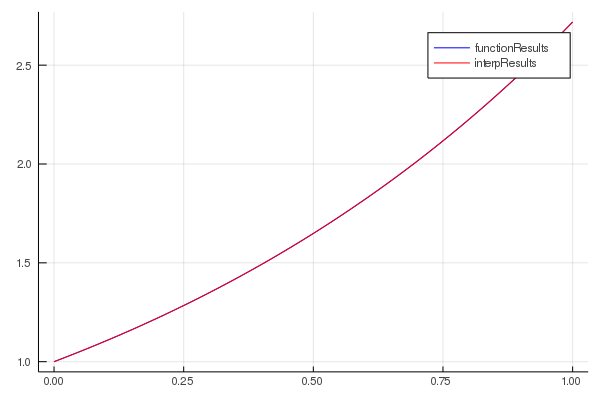
\includegraphics[scale=.4]{PLOT:0.0-1.0-5.png}
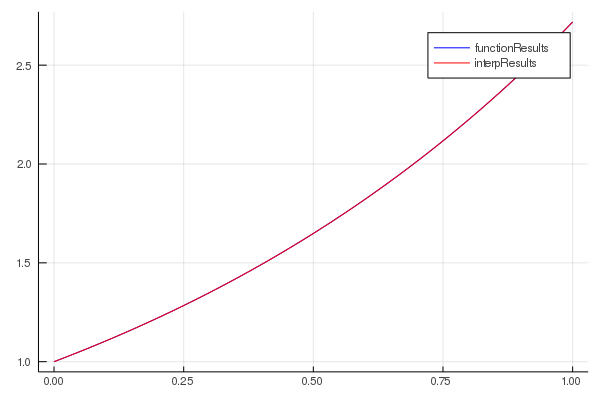
\includegraphics[scale=.4]{PLOT:0.0-1.0-10.png}
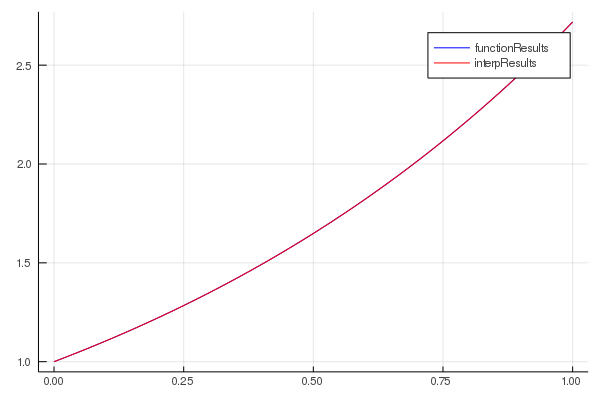
\includegraphics[scale=.4]{PLOT:0.0-1.0-15.png}
\end{figure}
\newpage
\subsubsection{b) $ x^2sin(x),[−1,1],n= 5,10,15$}
\begin{figure}[htbp]
\centering
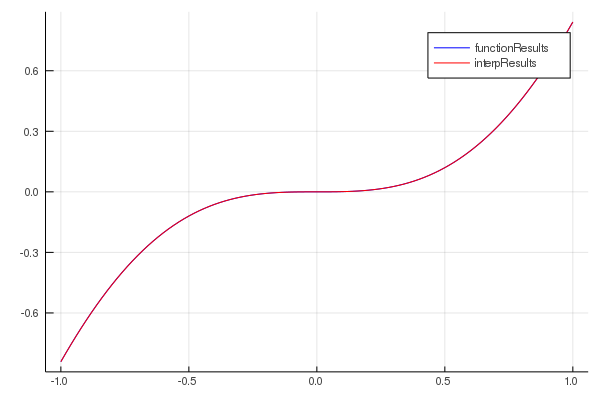
\includegraphics[scale=.4]{PLOT:-1.0-1.0-5.png}
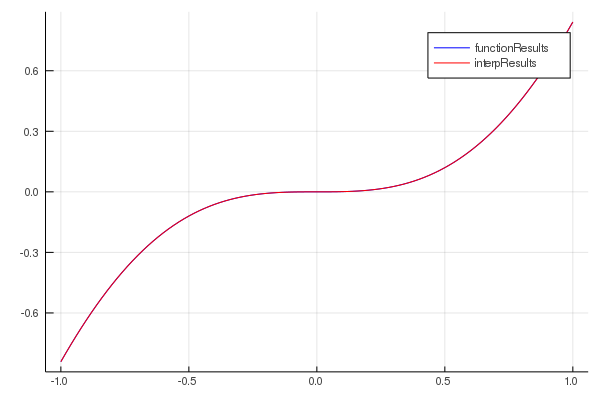
\includegraphics[scale=.4]{PLOT:-1.0-1.0-10.png}
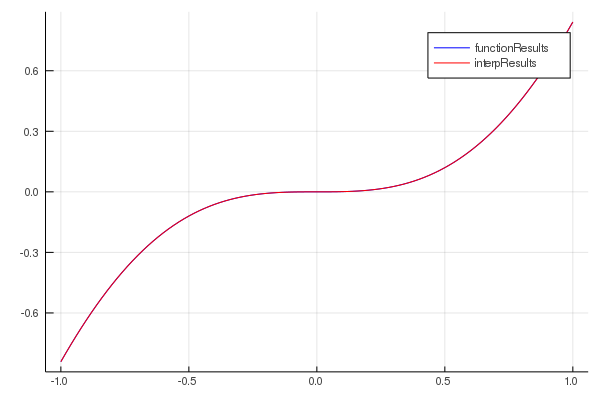
\includegraphics[scale=.4]{PLOT:-1.0-1.0-15.png}
\end{figure}

\subsection{Wnioski}
Jak widać w sekcji wyniki dla zadanych przykładów a i b wykresu wielomianów interpolacyjnych oraz interpolowanych funkcji są niemalże identyczne, nakładają się.\\ Wykorzystanie równoogległych węzłów przy interpoloacji dało niemal perfekcyjne wyniki. Powstałe wielomiany interpolacyjne praktycznie idealnie odwzorowały przebieg funkcji, co więcej zwiększenie stopnia wielomianu zwiększa jego podobieństwo do oryginalnej funkcji.

\newpage
\section{Zadanie 6}
\subsection{Opis Problemu}
\subsubsection{a) $|x|,[−1,1],n= 5,10,15$}
\subsubsection{b) $\dfrac{1}{1+x^2},[−5,5],n= 5,10,15 $ (zjawisko  Runge’go)}
\subsection{Rozwiązanie}
W celu rozwiązania zadania należy przetestować zaimplementowaną w Zadaniu 4 funkcję i narysować wykresy dla zadanych przykładów. Obserwacja Zjawiska Rozbieżności.
\subsection{Wyniki}
\subsubsection{a) $|x|,[−1,1],n= 5,10,15$}
\begin{figure}[htbp]
\centering
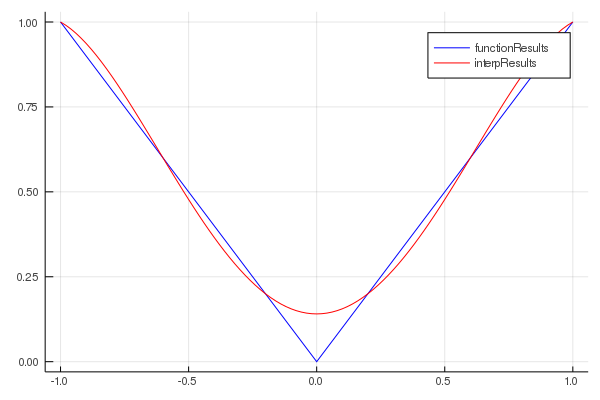
\includegraphics[scale=.4]{PLOT:-1.0|1.0|5.png}
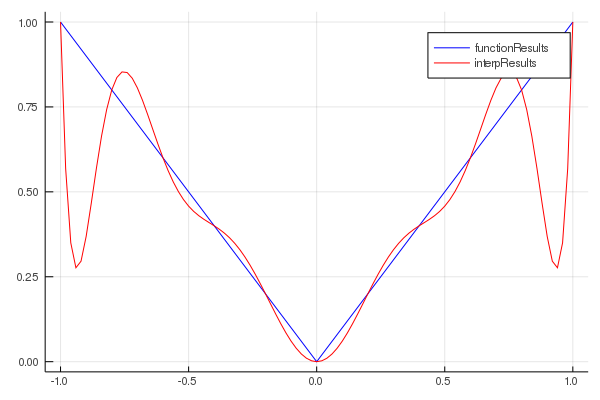
\includegraphics[scale=.4]{PLOT:-1.0|1.0|10.png}
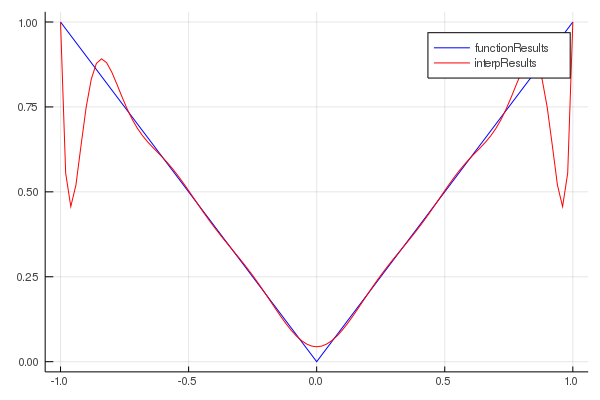
\includegraphics[scale=.4]{PLOT:-1.0|1.0|15.png}
\end{figure}
\newpage
\subsubsection{b) $\dfrac{1}{1+x^2},[−5,5],n= 5,10,15 $ (zjawisko  Runge’go)}
\begin{figure}[htbp]
\centering
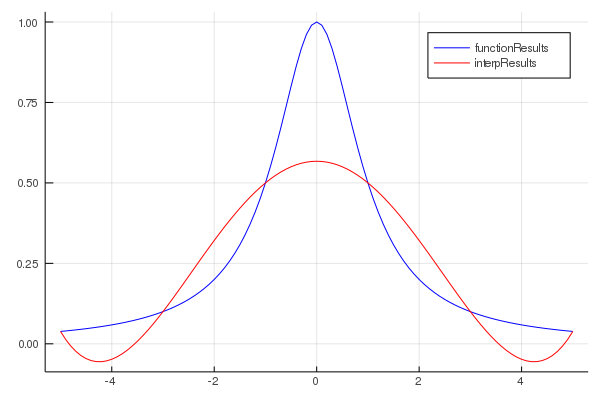
\includegraphics[scale=.4]{PLOT:-5.0|5.0|5.png}
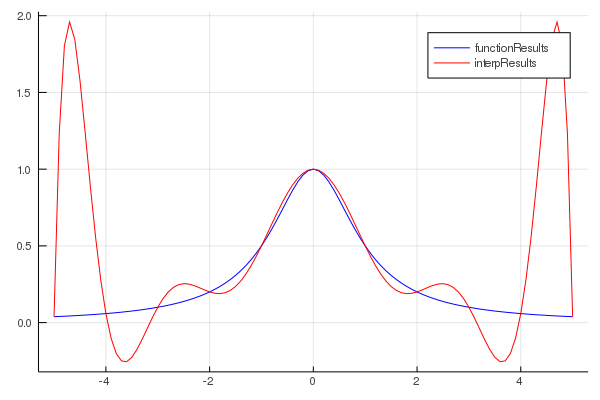
\includegraphics[scale=.4]{PLOT:-5.0|5.0|10.png}
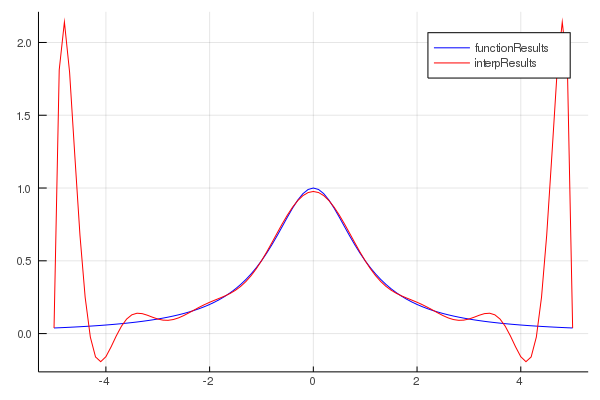
\includegraphics[scale=.4]{PLOT:-5.0|5.0|15.png}
\end{figure}
\newpage
\subsection{Wnioski}
\paragraph{Zjawisko Runge'go}
Wiąże się z zachowaniem  samych wielomianów bazowych: wielomiany oparte na węzłach równoodległych silnie oscylują w pobliżu krańców przedziału.\\
Na podstawie powyższych wyników jesteśmy w stanie zauważyć, iż wartości funkcji dla danych argumentów nie pokrywają się z wartościami wielomianów interpolacyjnch. Dla funkcji $|x|$ dziesie się tak, bo funkcja nie jest różniczkowalna. Natomiast funkcja $\dfrac{1}{1+x^2}$ jest przykładem powyżej wspomnianego zjawiska Runge'go. Zjawisko to występuje w przypadku pogorszenia jakości interpolacji wielomianowej pomimo zwiększenia ilości węzłow wielomianu interpolacyjnego. Przy zwiększaniu wartości n wykres początkowo sprawia złudzenie zmierzania do poprawnego kształtu, by po chwili całkowicie odejść od poprawności. Zjawisko jest popularne dla interpolacji za pomocą wielomianów wysokich stopni przy zastowaniu równoodległych węzłów. Występuje również w przypadku funkcji nieciągłej. W celu uniknięcia takiej sytuacji należy zastosowac interpolację z węzłami coraz gęściej upakowanymi na krańcach przedziału interpolacji.( Dobrym przykładem są wspomniane na stronie MIMUW węzły Czebyszewa, dla których wraz ze wzrostem sropnia wielomianu maleje błąd maksymalny aproksymacji funkcji). Wielomiany wysokiego stopnia nie są odpowiednim wyborem dla interpolacji dla równo oddalonych węzłów.
\end{flushleft}
\end{document}